\documentclass[10pt,twocolumn]{article}

\usepackage[T1]{fontenc}
\usepackage{lmodern}
\usepackage[letterpaper,top=0.8in,bottom=0.85in,left=0.75in,right=0.75in,columnsep=0.25in]{geometry}
\usepackage{amsmath,amssymb,amsthm}
\usepackage{graphicx}
\usepackage{xcolor}
\usepackage{booktabs}
\usepackage{array}
\usepackage{multirow}
\usepackage{microtype}
\usepackage{enumitem}
\usepackage{listings}
\usepackage{caption}
\usepackage{newfloat}
\DeclareFloatingEnvironment[fileext=lol,name=Listing]{listing}
\captionsetup{font=small,labelfont=bf,labelsep=period,justification=justified,singlelinecheck=off}
\usepackage{algorithm}
\usepackage{algpseudocode}
\usepackage{tikz}
\usetikzlibrary{arrows.meta,positioning,fit,calc,shapes.geometric,backgrounds}
\usepackage{pgfplots}
\pgfplotsset{compat=1.16}
\usepackage[numbers,sort&compress]{natbib}
\usepackage[hyphens]{url}
\Urlmuskip=0mu plus 1mu\relax
\def\UrlBreaks{\do\/\do\-\do\.\do\_}
\usepackage[colorlinks=true,linkcolor=blue!50!black,citecolor=blue!50!black,urlcolor=blue!50!black,
  pdftitle={Mwoyeo: In-Place Screen Translation that Keeps Up with the Scroll},
  pdfauthor={midagedev},pdfsubject={Mwoyeo method paper},pdfkeywords={screen translation, scroll prediction, text erasure}]{hyperref}

\setlist{nosep,leftmargin=1.4em}
\setlength{\parskip}{0pt}
\setlength{\emergencystretch}{2em}
\renewcommand{\topfraction}{0.9}
\renewcommand{\bottomfraction}{0.8}
\renewcommand{\textfraction}{0.08}
\renewcommand{\floatpagefraction}{0.75}
\renewcommand{\dblfloatpagefraction}{0.75}
\renewcommand{\dbltopfraction}{0.9}

\theoremstyle{plain}
\newtheorem{proposition}{Proposition}
\theoremstyle{definition}
\newtheorem{definition}{Definition}

% Swift listings, copied verbatim from the repository (see build.sh).
\lstdefinelanguage{Swift}{
  morekeywords={func,let,var,struct,enum,class,public,private,static,guard,else,if,return,for,in,where,case,switch,default,init,mutating,extension,import,some,as,is,nil,true,false,self,Self,try,throws,while,fileprivate},
  morecomment=[l]{//},
  morestring=[b]",
  sensitive=true
}
\lstset{
  language=Swift,
  basicstyle=\ttfamily\scriptsize,
  keywordstyle=\bfseries\color{blue!45!black},
  commentstyle=\itshape\color{black!60},
  stringstyle=\color{red!45!black},
  numbers=left,numberstyle=\tiny\color{black!55},numbersep=4pt,
  frame=tb,rulecolor=\color{black!40},
  columns=fullflexible,keepspaces=true,
  breaklines=true,breakindent=1.2em,breakautoindent=false,
  showstringspaces=false,
  aboveskip=0.4em,belowskip=0.2em,
  xleftmargin=1.6em
}
\lstdefinestyle{shell}{language={},basicstyle=\ttfamily\scriptsize,numbers=none,xleftmargin=0.4em}

% Notation.
\newcommand{\Real}{\mathbb{R}}
\newcommand{\code}[1]{\texttt{#1}}
\DeclareMathOperator{\clamp}{clamp}
\DeclareMathOperator{\median}{median}
\DeclareMathOperator{\MAD}{MAD}

\title{\bfseries Mwoyeo: In-Place Screen Translation\\that Keeps Up with the Scroll}
\date{2026-10-19}

\begin{document}

\twocolumn[
\begin{@twocolumnfalse}
\begin{center}
{\LARGE\bfseries Mwoyeo: In-Place Screen Translation\\[0.2em] that Keeps Up with the Scroll\par}
\vspace{1.1em}
\begin{tabular}{@{}p{0.31\textwidth}@{\hspace{0.015\textwidth}}p{0.31\textwidth}@{\hspace{0.015\textwidth}}p{0.31\textwidth}@{}}
\centering \textbf{midagedev}\\ Independent developer\\ \texttt{midagedev@gmail.com} &
\centering \textbf{The Mwoyeo project}\\ \texttt{github.com/midagedev/mwoyeo}\\ MIT licence, source revision \texttt{499e312} &
\centering \textbf{Correspondence}\\ \texttt{midagedev@gmail.com}\\ 2026-10-19
\end{tabular}
\vspace{1.0em}
\end{center}
\begin{center}
\begin{minipage}{0.86\textwidth}
\small
\textbf{Abstract.}\enspace
Reading a screen in another language usually means leaving it: a pop-up, a side panel, a subtitle bar.
Mwoyeo reads the text under a movable lens, erases it from the picture, and paints the translation back at the same place, in
the same size and colour. Doing this once is a pipeline. Doing it while the page scrolls is a timing problem, because every
stage works on a frame that the display has already left behind.
This paper describes the method as implemented at one revision of the open-source code.
Its core is a \emph{scroll predictor}: wheel and trackpad events become an expected content offset through a model of a delivery
latency $\lambda$, an ease-out step of length $T$ and a learnt ratio $\rho$ of content points per wheel unit; each captured
frame confirms the prediction, trains $\rho$, and is blended in by a critically damped spring.
Around it sit a robust background estimate with learned inpainting where the background is busy, and a rule set that decides
what must stay as written: formulas, identifiers, and code regions grouped by tint and indentation.
We state the equations and constants, and report what the benches kept in the repository measure: a probe-based translation
bench, a label-based keep bench, and a use-case bench of reading quality.

\end{minipage}
\end{center}
\vspace{0.8em}
\end{@twocolumnfalse}
]

\section{Introduction}\label{sec:intro}

A translation shown beside the text it translates asks the reader to look twice: once at the original, once at the
answer. A translation painted \emph{over} the original asks nothing, but it must be right in a stricter sense. The patch has to
cover exactly the old glyphs and nothing else, the new text has to fit the room the old text had, it has to look like the
page it sits on, and it has to stay put when the page moves. Mwoyeo\footnote{All code in this paper is copied from the
repository at revision \texttt{499e312} (2026-10-19), the main branch when the paper was written. Paths are relative to the
repository root; \texttt{sources.tsv} lists, for every number and every claim about the code, the file and line that carries
it, and \texttt{check.py} fails when one of them has moved.} is a macOS application that does this for the area under a
movable \emph{lens}.

The last requirement is the one that separates a demonstration from a tool. A lens over a chat or a feed is used while the
person scrolls it. The capture, the reading of the text, the translation and the repainting take time, so the translations
that arrive describe a frame that is already gone. Left alone they trail the text they translate by the speed of the scroll
times the age of the frame; the eye reads that as a shimmer, and in the worst case a translation sits on the wrong line.
That latency matters for direct manipulation is well established \citep{latency}.

\paragraph{Contributions.}
\begin{itemize}
\item A scroll predictor that places translations where the content will be by the time they are shown, from wheel and
  trackpad events alone, and that learns how far one wheel unit moves the page in the application under the pointer
  (Section~\ref{sec:scroll}). It is written as numbered equations, an algorithm and a 38-line listing, with a drift
  measure that the self-test prints.
\item A rule set for what must \emph{not} be translated: a formula or an identifier line, prose that is mostly inline mathematics,
  and regions of code, terminal output, logs, configuration and diffs found from tint, indentation and line-number gutters
  (Section~\ref{sec:keep}). The rules read text and geometry only; no model, no word list per language.
\item An erasure and re-setting stage built on a robust estimate of the background, with MI-GAN \citep{migan} where the
  background is not flat (Section~\ref{sec:erase}).
\item A description of how each part is measured in the repository's benches, with numbers taken only from result files
  that are committed there (Section~\ref{sec:measure}).
\end{itemize}

\paragraph{Scope.}
The paper describes what the code does at the stated revision, including what it does badly (Section~\ref{sec:limits}). Text
recognition runs in two places in this revision: document reads run in an XPC service, line reads still run in the
application's own process; moving the line reads into a second service is in progress and is not described as done.
We do not evaluate translation quality in general: the translation engines are interchangeable components, and the benches
here measure what the \emph{screen} adds to the problem.

\section{System overview}\label{sec:overview}

A person drags a rectangle, the \emph{lens}, over a chat, a feed or a game. The application keeps a screen capture of a
region that is larger than the lens, so that text next to the lens is already read, erased and translated when a drag or a
scroll brings it into view. Figure~\ref{fig:pipeline} shows the data path (blue) and the scroll path (orange).

\begin{figure*}[t]
\centering
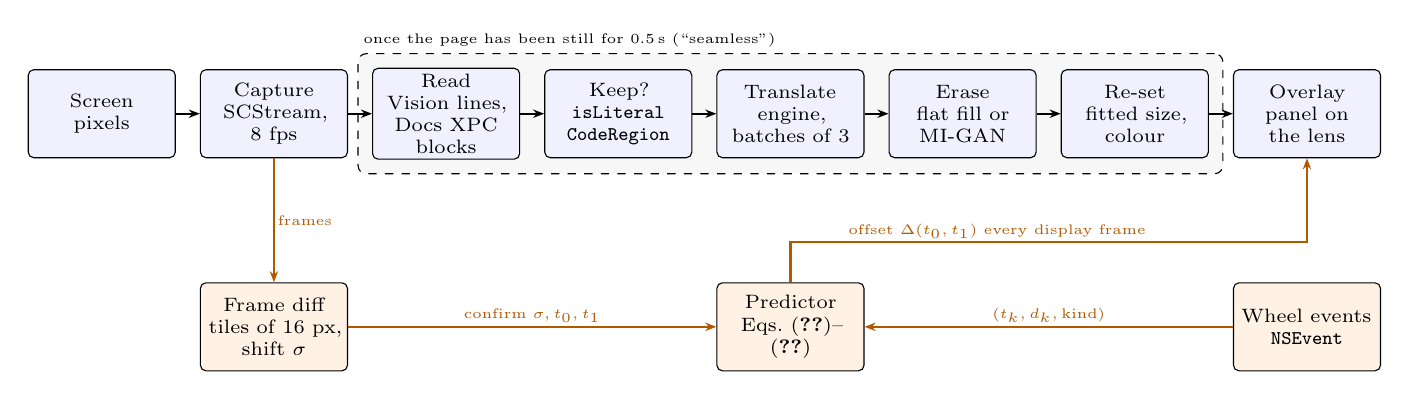
\begin{tikzpicture}[
  font=\scriptsize,
  box/.style={draw,rounded corners=2pt,fill=blue!6,minimum width=0.72in,minimum height=0.44in,text width=0.68in,align=center,inner sep=2pt},
  side/.style={draw,rounded corners=2pt,fill=orange!10,minimum width=0.72in,minimum height=0.44in,text width=0.68in,align=center,inner sep=2pt},
  flow/.style={-{Stealth[length=4pt]},thick},
  sig/.style={-{Stealth[length=4pt]},thick,orange!70!black},
  lab/.style={font=\tiny,inner sep=1pt,fill=white}
]
\node[box] (screen) {Screen\\ pixels};
\node[box,right=0.12in of screen] (cap) {Capture\\ SCStream,\\ 8 fps};
\node[box,right=0.12in of cap] (read) {Read\\ Vision lines,\\ Docs XPC blocks};
\node[box,right=0.12in of read] (keep) {Keep?\\ \code{isLiteral}\\ \code{CodeRegion}};
\node[box,right=0.12in of keep] (tr) {Translate\\ engine,\\ batches of 3};
\node[box,right=0.12in of tr] (erase) {Erase\\ flat fill or\\ MI-GAN};
\node[box,right=0.12in of erase] (set) {Re-set\\ fitted size,\\ colour};
\node[box,right=0.12in of set] (ov) {Overlay\\ panel on\\ the lens};
\foreach \a/\b in {screen/cap,cap/read,read/keep,keep/tr,tr/erase,erase/set,set/ov} \draw[flow] (\a) -- (\b);

\node[side,below=0.62in of cap] (diff) {Frame diff\\ tiles of 16 px,\\ shift $\sigma$};
\node[side,below=0.62in of tr] (pred) {Predictor\\ Eqs.~(\ref{eq:shown})--(\ref{eq:spring})};
\node[side,below=0.62in of ov] (wheel) {Wheel events\\ \code{NSEvent}};
\draw[sig] (cap) -- node[lab,right]{frames} (diff);
\draw[sig] (diff) -- node[lab,above]{confirm $\sigma,t_0,t_1$} (pred);
\draw[sig] (wheel) -- node[lab,above]{$(t_k,d_k,\text{kind})$} (pred);
\draw[sig] (pred.north) -- ++(0,0.2in) -| node[lab,pos=0.2,above]{offset $\Delta(t_0,t_1)$ every display frame} (ov.south);

\begin{scope}[on background layer]
\node[draw,dashed,rounded corners=3pt,fill=black!3,inner sep=0.07in,fit=(read)(set)] (seamless) {};
\end{scope}
\node[lab,anchor=south west,fill=none,inner sep=2pt] at (seamless.north west) {once the page has been still for 0.5\,s (``seamless'')};
\end{tikzpicture}

\caption{The pipeline. A captured frame is read into lines and blocks; blocks that must stay as written are dropped;
the rest are translated, their old glyphs erased, and the translation re-set at the same place. Orange: the scroll path.
Wheel events and the frame difference meet in the scroll predictor, which moves the finished blocks every display
frame.}\label{fig:pipeline}
\end{figure*}

\subsection{Capture and change detection}

The screen is captured with ScreenCaptureKit \citep{sckdoc}. The default rate is 8 frames per second, so the frame period is
$1/8 = 125$\,ms. The stream is configured with a minimum frame interval of one over the rate (capped at 30 frames per second)
and a queue depth of 4. Each frame is also reduced to a gray image. Two gray frames $a,b$ are compared tile by tile: a
$16\times16$ tile counts as changed when at least 2 of its pixels moved by more than 24 luma levels. Counting strong
changes, rather than averaging, keeps one edited glyph from being diluted by the rest of its tile and ignores compression
noise.

The pipeline works in two modes. While content moves, it re-reads only the changed band, shows each translation on a plain box
(``fast'') and follows scrolls by shifting existing blocks instead of reading them again. After the page has been still for
$0.5$\,s (the default \code{settleDelay}), it reads paragraphs, erases the source text and paints the translation in its place
(``seamless''), cross-fading from the plain boxes.

\subsection{Reading: lines and blocks}

Text is read with the Vision framework \citep{visiondoc}. A \emph{line} is what the line recogniser returns, with its
rectangle; a \emph{block} is a paragraph, the unit that is translated and repainted. Blocks come from one of two readers.
\begin{enumerate}
\item The \emph{document reader}, a document request of Vision that returns paragraphs, runs in its own XPC service (Docs) so
  that its model compilation, which can take tens of seconds the first time, never stalls the application. The lens does not
  wait for it: a pass that sends a request waits $S=2$\,s and then reads with the line reader while the request runs on.
  A document answer that is there when the line read ends is used; a later one marks the service ready and the lens reads
  once more.
\item The \emph{line reader} followed by a geometric paragraph grouper. The line reads run in the application's own process at
  this revision. The accurate recogniser has $S=3$\,s, the fast one $S=1$\,s.
\end{enumerate}
When successive slow answers show that the document reader is always late, the service is put to rest for $1,2,4,\dots,30$\,s
before the next request, so a service that is always slower than $S$ is not asked again by every recovery read.

\subsection{Translation}

The lines of a block are translated by an engine the person chooses: Apple's Translation framework \citep{transdoc} with a
language pack, or an engine added in the settings. Lines are sent in batches of at most three new lines in reading order.
By default nothing from the screen leaves the machine; text goes to a network engine only if the person adds one.

\subsection{Latency budget}

Table~\ref{tab:budget} lists the stages and the times that the repository records for them. They were measured on different
machines at different dates and are a budget, not a benchmark of the whole path.

\begin{table*}[t]
\centering
\caption{Stages of the data path, where each runs, and the time the repository records for it. The sources are in
\texttt{sources.tsv}.}\label{tab:budget}
\small
\begin{tabular}{@{}p{1.5in}p{1.75in}p{1.35in}p{1.9in}@{}}
\toprule
Stage & Runs in & Recorded time & Note\\
\midrule
Frame period & ScreenCaptureKit stream & $125$\,ms & default $8$ frames per second\\
Document read, warm & Docs XPC service & $0.33$--$0.48$\,s & patience $S=2$\,s derived from it\\
Line read, accurate, warm & application process & $0.25$--$0.88$\,s & patience $S=3$\,s ($\times3$ margin)\\
Line read, fast & application process & $0.06$--$0.10$\,s & Latin scripts only, $S=1$\,s\\
Translation, Apple low latency & on device & $0.15$\,s median per 3 lines & warm, M1 Pro (engine bench)\\
Inpainting, MI-GAN $512^2$ & GPU, Core ML & $13.3$\,ms median & M4 Pro, one patch (inpaint bench)\\
Settle before the seamless pass & timer & $500$\,ms & default \code{settleDelay}\\
Scroll prediction & main thread, display link & every display frame & no read, no model call\\
\bottomrule
\end{tabular}
\end{table*}

The last row is the point of Section~\ref{sec:scroll}. Every other row is a duration that a scroll cannot wait for: a frame
captured at time $t_0$ describes content that, by the time its translations are ready, has moved. The predictor spends no
read and no model call; it only adds up the events that the frame did not yet contain.

\section{What stays as written}\label{sec:keep}

An engine that is handed a fragment of a formula returns a sentence. The source of the formula test records a case: a figure label
``K'' came back from the engine as a word with a digit in it, and the overlay would then have painted that word over the typeset symbol. Some
text must therefore be recognised as \emph{not for translation} before any engine is asked. Two levels of rule do this: a rule
over one line or block (\code{TranslationFilter}), and a rule over a \emph{region} of blocks that sit together
(\code{CodeRegion}).

\subsection{Rules over one block}

Let $x$ be the text of a recognised line or block. The text is kept as written when
\begin{equation}\label{eq:literal}
\textit{literal}(x)\;=\;P(x)\,\lor\,F(x)\,\lor\,I(x)\,\lor\,H(x),
\end{equation}
where $P$ matches a fixed list of patterns (a shell prompt followed by a command, a time or date stamp, a URL or a bare
domain), $F$ is the formula test (\code{isFormula}), $I$ is the identifier test (a single word of at least three letters with a
lowercase letter directly followed by a capital: \code{MatMul}, \code{YouTube}) and $H$ is the mathematics-heavy test
(\code{isMathHeavy}). Table~\ref{tab:features} lists the features and thresholds.

\paragraph{The formula test.}
The line is cut into \emph{runs} of letters, digits and underscores; everything else is a sign. A \emph{prose word} is a run of
at least three letters with a vowel, or a contraction, that is not an \emph{operand}. Operands are the names of calls whose
arguments are variables (\code{Sublayer(x)}), the names of any call when the line holds an equals sign, and lowercase words
beside an equals sign. Let $L$ be the number of letters, $W$ the number of prose words, $\ell_w$ their letters and
$\ell_r=L-\ell_w$ the rest. A line is a formula when every letter is Latin, Greek or Cyrillic and
\begin{equation}\label{eq:formula}
F(x)\;=\;[L=1]\;\lor\;\bigl[\,W\le2\,\land\,\Lambda(x)\,\land\,\Sigma(x)\,\bigr],
\end{equation}
\begin{align*}
\Lambda\;=\;&(W{=}0)\;\lor\;(W{=}1\land e\land \ell_r\ge2\ell_w)\\
&\lor\;(W{=}2\land e\land c\land u\land 2\ell_r\ge3\ell_w).
\end{align*}
Here $e$ says that the line holds a relation sign, $c$ that it holds a call, and $u$ that the two prose words are its first two
runs: one or two words of prose among many symbols are the label of a typeset line (``where $\mathrm{head}_i$ =
Attention(\dots)''). $\Sigma$ is the evidence of mathematics: a sign (an operator, an arrow, a super- or subscript, a Greek
letter used as a symbol, an underscore in a name, a call, a run that mixes Latin and Cyrillic, which is how an OCR misreads
a sign), or a line that has only atoms (no run of two letters with a vowel) and holds a digit-letter run (\code{x1}) or a
capital consonant cluster without digits (\code{QKT}); a short Cyrillic fragment beside a bracket is a third form of the same misreading.

\paragraph{Prose that is mostly mathematics.}
A block of prose with inline formulas, read off a typeset page, comes back garbled, and a translation would only set garbled
symbols between a few translated words. The block stays as written when the share of its letters and digits that are
mathematics is high:
\begin{equation}\label{eq:share}
H(x)\;=\;\Bigl[\tfrac{n_{\mathrm{math}}}{n_{\mathrm{math}}+n_{\mathrm{prose}}}\ge0.30\Bigr]\land\bigl[k_{\mathrm{sign}}\ge2\bigr]\land\bigl[n\ge20\bigr],
\end{equation}
with $n=n_{\mathrm{math}}+n_{\mathrm{prose}}$. Mathematics are signs, variables of one letter (not ``a'' and ``I''), runs of consonants or with an inner capital, names with an
underscore, numbers beside a sign, and any word beside a sign. Prose is a word of three letters or more with a vowel and no inner
capital that stands beside no sign. Numbers, names of letters with digits, two-letter words and punctuation are neutral. A
currency sign next to a number is a price and not a sign.

\begin{table*}[t]
\centering
\caption{Features and thresholds of the keep rules. The first block is over one line or block, the second over a region.
Heights are median line heights of a block. The line of the source that carries each value is in \texttt{sources.tsv}.}\label{tab:features}
\small
\begin{tabular}{@{}p{0.95in}p{1.45in}p{4.2in}@{}}
\toprule
Rule & Feature & Definition and threshold\\
\midrule
\code{isFormula} & single letter & one letter in the line: a formula\\
 & prose words & at most 2; with 1: relation and $\ell_r\ge2\ell_w$; with 2: first two runs, relation, call and $2\ell_r\ge3\ell_w$\\
 & operand & a call name with variable arguments; any call name when the line has an equals sign; lowercase beside an equals sign\\
 & signs & \texttt{=\ \^{}}\ $\pm\ {}^2\ {}^3\ {}^1\ \times\ \div$, sub- and superscripts, arrows, U+2200--22FF, Greek used as a sign, \code{\_}, a call\\
\midrule
\code{isMathHeavy} & share of mathematics & $\ge 0.30$ of letters and digits\\
 & signs / size & at least 2 signs and at least 20 letters and digits\\
\code{isIdentifier} & camelCase & letters only, at least 3, a lowercase letter then a capital\\
\midrule
\code{CodeRegion} & tint & background differs from the frame's by $\ge6$ levels in a channel\\
 & neighbours & stacked within $1.5\,h$, or side by side on one row within $3.0\,h$\\
 & indentation & left edge $\ge0.75\,h$ right of its column's margin; the margin is sought among blocks within $25\,h$\\
 & keywords & strong count $\ge1$, strong $+\,0.5\,\cdot$ weak $\ge1.5$, and keywords $\ge0.2$ of the tokens\\
 & line ends & $\ge0.4$ of the lines end in \code{; \{ \} ) ]}, at least one in \code{; \{ \}}\\
 & symbols & $\ge0.15$ of at least 6 printable ASCII characters (spaces excluded) are code symbols\\
 & density & from 4 content blocks, at least $0.3$ of them show a text feature\\
\bottomrule
\end{tabular}
\end{table*}

\subsection{Rules over a region}\label{sec:region}

A block of text alone often does not show that it is code. A document read cuts a listing into one-line blocks, and
\code{end if} means nothing by itself. \code{CodeRegion} therefore works on a region: the blocks of one read that sit together in
one box, one indented run or one line-number gutter. Its evidence is of two kinds. A \emph{container} says that blocks belong
together: a tint that differs from the frame's, an indented run, a gutter. \emph{Text} features say what the blocks hold:
keywords, line ends, symbols, a comment marker, a prompt, a hash-led line, diff marks, an assignment. A container alone keeps
nothing, because a callout box, a bullet list and a table are containers of prose; text alone keeps only when it is strong.

Let each block $i$ have a rectangle $[x^0_i,x^1_i]\times[y^0_i,y^1_i]$, a line height $h_i$ (the median of its line heights) and a
word count $w_i$. The block is \emph{tinted}, $\tau_i=1$, when its background colour differs from the frame's by at least $6$
levels in a channel. It is \emph{indented}, $\iota_i=1$, when
\begin{equation}\label{eq:indent}
\iota_i=\bigl[\,x^0_i-m_i\ge0.75\,h_i\,\bigr],\qquad m_i=\min\bigl(\{x^0_i\}\cup M_i\bigr),
\end{equation}
where $M_i$ holds the $x^0_c$ of the blocks $c$ with $w_c\ge2$ that overlap $i$ in $x$ and whose middle lies within $25\,h_i$ of the middle of $i$ vertically.
Two blocks are \emph{linked} when they are neighbours and share a tint, an indent or a gutter:
\begin{equation}\label{eq:link}
\begin{aligned}
i\sim j\iff{}&\mathrm{near}(i,j)\land\bigl[\,\tau_i\tau_j\,[\delta(b_i,b_j)\le6]\ \lor\ \iota_i\iota_j\\
&\lor\ (g_i\lor g_j)\,\mathrm{row}(i,j)\ \lor\ g_ig_j\,\bigr],
\end{aligned}
\end{equation}
where $\delta$ is the largest channel difference of the two background colours $b_i,b_j$, $g_i$ says that the block is a
line-number gutter, $\mathrm{row}(i,j)$ that the blocks overlap vertically by more than half of $h=\min(h_i,h_j)$, and
$\mathrm{near}$ holds when the blocks are stacked within $1.5\,h$ and overlap in $x$, or sit on one row within $3.0\,h$.
Regions are the connected components of $\sim$, found with a union--find.

Let $R$ be a region, $S$ the number of \emph{strong} features that its lines show (keyword, line end, comment, prompt, log
line, diff), and $A$ the number of all features, including the weak ones (symbol, assignment). With $T=\max_i\tau_i$ and the
container $C=T\lor\bigl(|R|>1\land\forall i\,(\iota_i\lor g_i)\bigr)$, the region is kept when
\begin{equation}\label{eq:verdict}
\begin{aligned}
\mathrm{keep}(R)\;=\;&\Bigl[\,T\,(S\ge1\lor A-S\ge2)\ \lor\ C\,[S\ge1]\\
&\lor\ \bigl(|R|>1\land S\ge1\land A\ge2\bigr)\\
&\lor\ \mathrm{prompt}\ \lor\ S\ge2\,\Bigr]\ \land\ D(R),
\end{aligned}
\end{equation}
where $D(R)$ is the density test of Table~\ref{tab:features}: a long region needs a text feature in a share of its content blocks,
so one stray \code{end} in a page-wide indented run keeps nothing. The reason attached to a kept region is, in this order,
terminal (a prompt), diff, log, configuration (an assignment with no keyword and no line end) and otherwise code. Listing~\ref{lst:verdict}
is the function.

\begin{listing}[t]
\lstinputlisting[firstnumber=251]{listings/CodeRegion_verdict.swift}
\caption{\code{CodeRegion.verdict}, \texttt{Core/Sources/MwoyeoCore/CodeRegion.swift}, lines 251--267, as it is in the
repository.}\label{lst:verdict}
\end{listing}

Everything in this section reads text, geometry and the background colour only. There is no model and no list of words per language: a comment in any
script is code because of where it sits. The constants were fitted on the development sets of the keep-label bench and
checked on held-out sets (Section~\ref{sec:measure}).

\section{Erasing and re-setting the text}\label{sec:erase}

For each block that is kept for translation, the old glyphs are removed from the picture and the translation is drawn
into the place they left. The stage has three parts: a mask of the glyph pixels with an estimate of the background and the
text colour, a fill (flat, or learned where the background is busy), and a fit of the translation to the room the old text had.

\subsection{Mask, background and colour}

For every line of the block the stage crops the line's rectangle with a ring of $r=\max(3,\lfloor0.18\,h\rfloor)$ pixels around it,
where $h$ is the line height. The ring is the background sample. Let $\ell(p)$ be the luma of pixel $p$ and $\tilde\ell$ the median
luma of the ring. The noise of the background is the robust spread of the ring,
\begin{equation}\label{eq:mad}
\hat\sigma\;=\;1.4826\;\median_{p\in\text{ring}}\bigl|\ell(p)-\tilde\ell\bigr| ,
\end{equation}
where the factor makes the median absolute deviation consistent with the standard deviation of a Gaussian \citep{mad}. A median
instead of a mean keeps a box edge, or a bit of another element of the page that falls in the ring, from skewing the estimate.
The background is \emph{flat} when $\hat\sigma<6$. The background colour is the per-channel median of the ring.

Glyph pixels are one of the two classes of Otsu's threshold \citep{otsu},
\begin{equation}\label{eq:otsu}
t^\star\;=\;\arg\max_t\ \omega_0(t)\,\omega_1(t)\,\bigl(\mu_0(t)-\mu_1(t)\bigr)^2 ,
\end{equation}
computed on the luma histogram of the text rectangle: the class on the side away from the background. A pixel is a candidate when
it is in that class and $|\ell(p)-\tilde\ell|\ge\max(12,\lfloor2.5\,\hat\sigma\rfloor)$. Candidates are grouped into 8-connected components, and a
component is kept only when it reaches into the text rectangle and does not run off the outer edge of the crop where a ring
exists: glyphs sit inside the ring, while box borders and rules continue past it. The mask is dilated by
$\max(1,\lfloor0.07\,h\rfloor)$ pixels to swallow the anti-aliased edges, and enclosed holes are filled. If segmentation fails (the
glyph class covers more than $0.6$ of the text rectangle, or there is none) the whole rectangle is the mask.

The text colour is the mean colour of the half of the glyph pixels that contrast most with the background, because edge pixels
are blended with it. Outlined text, such as video subtitles, has two tones, and either one alone would leave the other behind:
the mask then takes both, and the outline colour is kept for the translation. Coloured frames drawn round glyphs, such as the
box a viewer draws round a link, are taken into the mask when they are thin outlines that hold glyph pixels inside.

\subsection{Fill and inpainting}

If the background of every line of the block is flat, or inpainting is turned off, the masked pixels are filled with the
background colour. Otherwise the patch is repaired with MI-GAN \citep{migan}, a generator designed for inpainting on mobile
devices. The model takes a $4\times512\times512$ tensor whose first channel is $M-\tfrac12$, with $M=1$ for known pixels and $M=0$ for the
hole, and whose other channels are the RGB values scaled to $[-1,1]$ and multiplied by $M$. Its output is a full-frame
reconstruction $G$ that also differs from the input outside the hole, so the result is composited:
\begin{equation}\label{eq:composite}
\hat I\;=\;M\odot I\;+\;(1-M)\odot G\bigl(M-\tfrac12,\ M\odot I\bigr).
\end{equation}
A rectangle larger than a window is tiled with $512\times512$ windows at a step of $\tfrac34\cdot512=384$ pixels, each window centred on its
tile and taking real frame pixels as context; only hole pixels inside the tile are written.

Core ML runs the model on the CPU, the GPU or the Neural Engine. The inpaint bench measured the three on a $512^2$ patch
(Table~\ref{tab:migan}), and the application selects the GPU: the default setting that lets Core ML choose among all units was four
times slower there. The 14.2\,MB model is not loaded at launch; it loads at the first fill, and is released after 60\,s without one.

\begin{table}[t]
\centering
\caption{MI-GAN $512^2$ prediction time by compute unit, one patch, median of 20 timed runs after 3 warm-up runs (inpaint bench,
M4 Pro).}\label{tab:migan}
\small
\begin{tabular}{@{}lrr@{}}
\toprule
Compute unit & Median (ms) & p90 (ms)\\
\midrule
CPU only & 212.5 & 320.5\\
CPU and GPU & 13.3 & 13.4\\
CPU and Neural Engine & 20.0 & 20.3\\
All units & 55.3 & 64.1\\
\bottomrule
\end{tabular}
\end{table}

\subsection{Re-setting the translation}

The translation is laid out in the room of the old text, and the room can be larger than the old text: free background to the
right of the block is part of the patch, up to $80\%$ of the block's width and up to the edge of its column, where free means
that no pixel differs from the background colour by more than $22$.

\paragraph{Size.}
The size of the old text is read from the height $h_g$ of its glyphs: the em size is $h_g/0.88$ for Chinese, Japanese and
Korean text, whose glyphs fill about $88\%$ of the em, and for Latin text $h_g/0.72$ (cap height) or $h_g/0.95$ when the text has
descenders. The translation is then set at the largest size that fits the room. With $\mathrm{measure}(s)$ the size of the laid-out
text at font size $s$,
\begin{equation}\label{eq:fit}
s^\star\;=\;\max\bigl\{\,s\in[s_{\min},s_{\max}]\ :\ \mathrm{measure}(s)\le\mathrm{box}\,\bigr\},
\end{equation}
which is found by bisection to a resolution of $0.5$ pt (\code{TextFitter.fitFontSize}); when nothing fits, $s_{\min}$ is returned and
the caller wraps the text or lets it overflow. As a last resort a translation that does not fit at the smallest size is cut at a
word boundary and ends in an ellipsis. The ellipsis is counted by the paper bench (Section~\ref{sec:measure}), because it is a
loss: the person reads a shorter sentence than the engine returned.

\paragraph{Place and colour.}
The text starts where the old text started: the patch reaches the erase margin $r$ past the original on every side, and the text
area is the original block. The text colour is the sampled colour above, the background is the repaired patch, and Hangul syllables
of a word are joined with a word joiner so that the platform's line breaker does not split a word between two syllables.

\section{Scroll prediction}\label{sec:scroll}

A lens over a feed is used while the feed scrolls. At the default rate the screen is captured every $125$\,ms, and the blocks that
are placed from a frame captured at $t_0$ are shown at a later display time $t$. If the content has moved by $X(t)-X(t_0)$
points in between, an unpredicted block is that far from the text it translates. At a scroll speed of $v=1000$ points per second a
frame that is only $125$\,ms old is $v\cdot0.125=125$ points off, several lines of text. The reading and the translation of a
frame take longer than that. Moving the finished blocks along with the page is therefore not an optimisation; without it the
overlay is wrong whenever the page moves.

\subsection{Model}

The application cannot ask a page how far it has scrolled, and does not need to. It sees a scroll event anywhere on the screen
(whether it scrolls what a lens reads is decided afterwards), and the system sends it with a time stamp, a signed delta $d$ in the units of the device, and a flag
that says whether the deltas are \emph{precise} (a trackpad: points, which browsers apply one to one) or \emph{lines} (a mouse wheel:
the application decides how many points a line is, and usually animates the step). Momentum scrolling needs nothing special: the
system keeps sending events that decay.

The predictor keeps the events of the last 2\,s as triples $(t_k,d_k,c_k)$ with $c_k\in\{P,L\}$ (precise, lines), positive $d$
moving the content down.\footnote{The sign convention is that of the source: a positive delta moves content down (\texttt{ScrollPredictor.swift}, the comment of \texttt{wheel}). Reading down a page moves its content up, which is a negative delta, as in the examples of Appendix~\ref{app:examples}.} Two constants describe the path from an event to the screen: a delivery latency $\lambda=16$\,ms,
and the duration $T=150$\,ms over which an application animates one line step. The fraction of event $k$ that is on screen at time $t$ is,
with $s=t-t_k-\lambda$,
\begin{equation}\label{eq:shown}
\varphi_k(t)\;=\;\begin{cases}
0 & s\le0,\\
1 & s>0,\ c_k=P,\\
1-\bigl(1-\min(1,s/T)\bigr)^3 & s>0,\ c_k=L.
\end{cases}
\end{equation}
A precise delta is a step: the content has moved all at once. A line step eases out, as in a smooth-scroll animation: it starts at
speed $3/T=20\ \mathrm{s}^{-1}$ of its total and slows to zero at $T$, so that half of it is on screen after $T(1-2^{-1/3})\approx31$\,ms, ninety percent
after $T(1-0.1^{1/3})\approx80$\,ms, and all of it after $T=150$\,ms.

\begin{figure}[t]
\centering
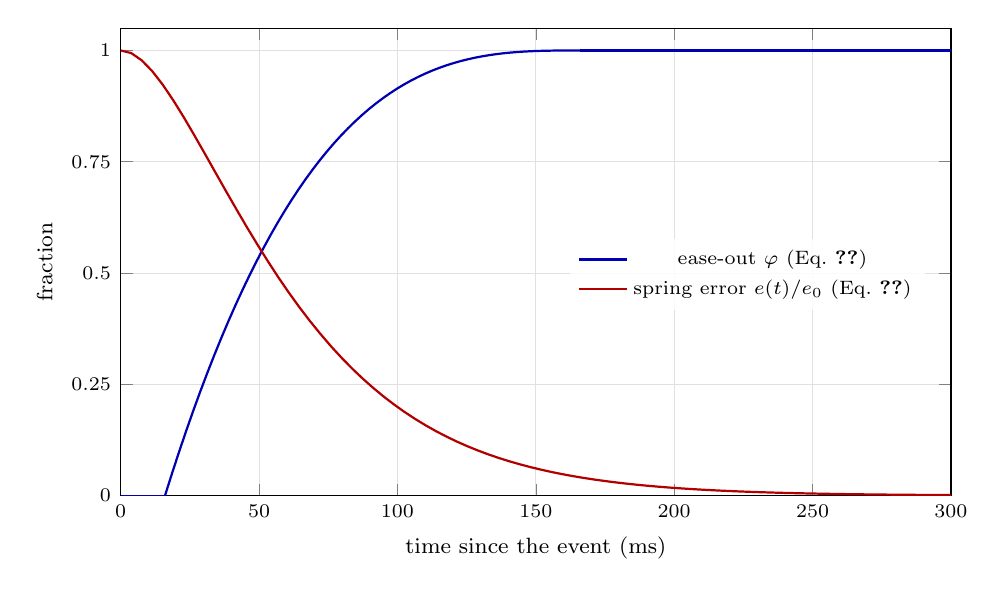
\begin{tikzpicture}
\begin{axis}[
  width=\columnwidth,height=0.62\columnwidth,
  xlabel={time since the event (ms)},ylabel={fraction},
  xmin=0,xmax=300,ymin=0,ymax=1.05,
  xtick={0,50,100,150,200,250,300},ytick={0,0.25,0.5,0.75,1},
  tick label style={font=\scriptsize},label style={font=\footnotesize},
  legend style={font=\scriptsize,at={(0.97,0.55)},anchor=north east,draw=none,fill=white,fill opacity=0.85,text opacity=1},
  grid=major,grid style={black!12},
  every axis plot/.append style={thick}
]
\addplot[blue!70!black,domain=16:166,samples=60] {1-(1-(x-16)/150)^3};
\addlegendentry{ease-out $\varphi$ (Eq.~\ref{eq:shown})}
\addplot[blue!70!black,forget plot] coordinates {(0,0) (16,0)};
\addplot[blue!70!black,forget plot,domain=166:300,samples=2] {1};
\addplot[red!70!black,domain=0:300,samples=80] {(1+0.03*x)*exp(-0.03*x)};
\addlegendentry{spring error $e(t)/e_0$ (Eq.~\ref{eq:spring})}
\end{axis}
\end{tikzpicture}

\caption{The two curves of the model, plotted from the equations, not measured: the fraction of a line step on screen
(Eq.~\ref{eq:shown} with $\lambda=16$\,ms, $T=150$\,ms) and the decay of a correction (Eq.~\ref{eq:spring}).}\label{fig:curves}
\end{figure}

\subsection{Offset between two frames}

The wheel units of kind $c$ that reached the screen between $t_0$ and $t_1$ are
\begin{equation}\label{eq:units}
U_c(t_0,t_1)\;=\;\sum_{k:\ c_k=c} d_k\,\bigl[\varphi_k(t_1)-\varphi_k(t_0)\bigr],
\end{equation}
and the content movement expected between them, in points, is
\begin{equation}\label{eq:offset}
\Delta(t_0,t_1)\;=\;\rho_P\,U_P(t_0,t_1)\;+\;\rho_L\,U_L(t_0,t_1).
\end{equation}
The ratios $\rho_c$ are points per wheel unit. $\rho_P$ starts at $1$; $\rho_L$ is unknown, and contributes $0$, until a frame has shown
how far a line goes. A display tick at time $t$ moves every block of the scroll area, which the frame $t_0$ placed, by $\Delta(t_0,t)$.

Two properties follow from the form of Eq.~(\ref{eq:units}), and the second is why the predictor needs no state beyond the
events.

\begin{proposition}[Exact tracking]\label{prop:exact}
If every event is precise, $\rho_P=1$, $\lambda=0$ and the application moves the content by exactly $d_k$ at $t_k$, then
$\Delta(t_0,t_1)=\sum_{t_0\le t_k<t_1}d_k=X(t_1)-X(t_0)$.
\end{proposition}

\begin{proposition}[Re-basing]\label{prop:rebase}
For $t_0\le t_1\le t$ and fixed ratios, $\Delta(t_0,t)=\Delta(t_0,t_1)+\Delta(t_1,t)$.
\end{proposition}

\noindent Both are one line: $\varphi_k(t_1)-\varphi_k(t_0)$ is a difference, and the differences telescope. The first is a unit
test (ten events of $-4$ points, the frame placed in the middle of them: five are left and $\Delta=-20$). The second means that when
the next frame, captured at $t_1$, contains the movement up to $t_1$, the display only has to add $\Delta(t_1,t)$: nothing is
counted twice and nothing is lost at the frame boundary. It also means that a wrong ratio produces an error that the next frame
can measure.

\subsection{What the frame confirms}

Each captured frame is compared with the previous one. A band of columns that changed is matched against the previous frame by the
mean absolute difference of its gray pixels over the rows that overlap after a shift $d$,
\begin{equation*}
\mathrm{err}(d)\;=\;\frac1{|\Omega_d|}\sum_{(x,y)\in\Omega_d}\bigl|a(x,y)-b(x,y+d)\bigr| ,
\end{equation*}
sampling every other column. The shift is searched over whole pixels, at most a quarter of the band's height, and then refined by $\pm0.5$ and $\pm0.25$ with the two nearest
rows of $b$ blended, so smooth scrolling is resolved to a quarter of a pixel of the downsampled image. It is accepted only when
$|d|\ge0.25$, $\mathrm{err}(d)<0.6\,\mathrm{err}(0)$ and $\mathrm{err}(d)<8$. A band too plain to be matched on its own takes its
neighbour's shift if that explains it better than no move; neighbouring bands whose shifts differ by at most $0.5$ form one
\emph{region}, and a region shorter than three tiles is something moving in place, not a scroll. Pages keep fixed parts (headers,
sidebars, an input box) beside the part that scrolls, which is why the match is made per column band and not for the whole frame.

A region that holds the pointer yields a \emph{report}: the shift $\sigma$ in points (positive = down) and the capture times $t_0,t_1$ of
the two frames. The predictor learns from it. Let $u_P=U_P(t_0,t_1)$ and $u_L=U_L(t_0,t_1)$. The report is used only if exactly one of
$|u_P|,|u_L|$ is at least one unit (it cannot tell two ratios apart from one shift). With $c$ the kind that has units, the sample is
$\hat\rho=\sigma/u_c$ and
\begin{equation}\label{eq:confirm}
\rho_c\;\leftarrow\;\begin{cases}
\hat\rho & \rho_c\ \text{unknown},\\
\rho_c+0.3\,(\hat\rho-\rho_c) & 0.33<\hat\rho/\rho_c<3,\\
\rho_c & \text{otherwise,}
\end{cases}
\end{equation}
where the first case also needs $\hat\rho$ finite and nonzero. The gate around $\rho_c$ ignores what says nothing: a stop at the end of the page (events but no movement), or a scroll by other means (keys, scripts). In the
unit test, fifty precise units with a ratio of $1$ meet a frame that shows $-60$ points: $\hat\rho=1.2$, the ratio becomes $1+0.3\cdot0.2=1.06$ and the
next offset for the same events is $-53$. Without noise, the error of $\rho_c$ shrinks by the factor $0.7$ with every accepted
report, to $17\%$ after five and $2.8\%$ after ten. The ratio belongs to the application and page under the pointer, so it is forgotten when
a new gesture starts over a different window.

The prediction is used only while events keep coming: the overlay asks for $\Delta$ only if the last event is less than
one second old and a scroll area is known (first guessed as the lens's part of the window under the pointer, and
corrected by the first frame that moves).

\subsection{Correcting the display}

When the next frame arrives, the blocks it has moved are where the content is, and the blocks the display showed were where the
prediction put them. The difference $e$ is an error of the prediction, and a jump of $e$ would show as a jolt. If $|e|<80$ points the layer
is given an additive spring animation from $e$ to $0$ with mass $m=1$ and stiffness $k=900$, and the damping is set to the critical value
$c=2\sqrt{km}=60$. With $\omega_0=\sqrt{k/m}=30$ rad/s and zero initial velocity (the default of the animation, which the code does not
set), the remaining error is
\begin{equation}\label{eq:spring}
e(t)\;=\;e_0\,(1+\omega_0t)\,e^{-\omega_0t},
\end{equation}
which has no overshoot. It is down to $5\%$ of $e_0$ after $158$\,ms and to $1\%$ after $221$\,ms. A correction that is still easing in when
the next one arrives carries on from where the block is seen, not from where it was going. Ending a prediction, when the events stop, is a correction too:
whatever the frames have not confirmed eases away.

\begin{algorithm}[t]
\caption{Predict and correct, per lens.}\label{alg:predict}
\begin{algorithmic}[1]
\Procedure{OnWheel}{$e$}
  \If{$e$ starts a gesture over another window} \State reset $\rho_P\gets1$, $\rho_L\gets\bot$, forget the events \EndIf
  \State append $(t_e,d_e,c_e)$, drop events older than 2\,s
  \State $t_\ell\gets t_e$
\EndProcedure
\Procedure{OnTick}{$t$}\Comment{every display frame}
  \If{$t-t_\ell<1$\,s \textbf{and} the scroll area is known} \State $\Delta\gets\rho_PU_P(t_f,t)+\rho_LU_L(t_f,t)$
  \Else\ \State $\Delta\gets0$ \EndIf
  \ForAll{block $b$ in the scroll area}
    \State $e\gets\mathrm{shown}_b-(y_b+\Delta)$; \ $\mathrm{shown}_b\gets y_b+\Delta$
    \If{correcting \textbf{and} $0<|e|<80$} \State add a critically damped spring \EndIf
  \EndFor
\EndProcedure
\Procedure{OnFrame}{frame at $t_1$, previous frame at $t_0$}
  \ForAll{scroll region $r$ with shift $\sigma$}
    \State move the blocks in $r$ by $\sigma$
    \If{$r$ holds the pointer} \State confirm$(\sigma,t_0,t_1)$ by Eq.~(\ref{eq:confirm}) \EndIf
  \EndFor
  \State $t_f\gets t_1$; \ \Call{OnTick}{now} with correcting
\EndProcedure
\end{algorithmic}
\end{algorithm}

\subsection{Drift}

The quantity that matters is how far a shown translation is from the text it translates. The self-test measures it. For each block it records, when the
block is first seen, its position on the \emph{page}: the on-screen position plus the scroll offset for blocks inside the scrolling rectangle. At
every captured step $f$ it takes the largest displacement of any shown block from that anchor,
\begin{equation}\label{eq:drift}
D_f\;=\;\max_{b\in B_f}\ \bigl\|p_b(f)-p_b(0)\bigr\|_2,
\end{equation}
and prints $D_f$ per frame and, at the end, the mean of $D_f$, the maximum, and the number of frames with $D_f>2$ points. A block that is re-laid out is
anchored again. With exact prediction every block stays on its text and $D_f=0$ (Proposition~\ref{prop:exact}); without it, $D_f$ is the distance the page has moved since the frame the block was placed from. In the
self-test the application is simulated with $\lambda=0$ and wheel deltas equal to the true scroll, which is the best case for the predictor: drift there isolates what the pipeline adds, and a real application
adds its own animation and the error of $\rho$ on top.

Listing~\ref{lst:scroll} is the predictor. It has no dependency on the system: it takes times as numbers, which is how the unit tests drive it.

\begin{listing*}[t]
\lstinputlisting[firstnumber=31]{listings/ScrollPredictor_core.swift}
\caption{The core of \code{ScrollPredictor}, \texttt{Core/Sources/MwoyeoCore/ScrollPredictor.swift}, lines 31--68 (\code{offset},
\code{confirm}, \code{reset}, \code{units}, \code{shown}), as it is in the repository. \code{shown} is Eq.~(\ref{eq:shown}),
\code{units} Eq.~(\ref{eq:units}), \code{offset} Eq.~(\ref{eq:offset}) and \code{confirm} Eq.~(\ref{eq:confirm}).}\label{lst:scroll}
\end{listing*}

\section{Measurement}\label{sec:measure}

The repository keeps four benches under \texttt{tools/}. Each is built to block one failure mode, and each has a scorer that is a
script. The numbers in this section come only from result files that are committed in the repository; each table says which. Where
a bench has no committed result for a claim, the text says so.

\subsection{Use-case bench: was the text read as a unit?}

\texttt{tools/usecase-bench} renders 52 scenes in six use cases, drawn from HTML written for the bench, with the scene
dimensions in \texttt{set/index.tsv}: 5 chats, 11 documents and web pages, 8 game screens, 7 papers, 9 subtitle frames and 12 code
scenes. For each scene a file lists the \emph{units} that a reader should return as one block (a paragraph, a table cell, a
title): 400 units in all (36 in chats, 89 in documents, 38 in games, 70 in papers, 20 in subtitles, 147 in code). A rendered scene is read, and
every unit gets one of five outcomes:
\emph{correct} (the unit is exactly one block), \emph{merged} (it is inside a longer block), \emph{split} (it is cut into pieces that
together cover at least $80\%$ of it), \emph{misread} (the best block is at least $0.75$ similar) and \emph{missing}. Eighty of the units are marked
as \emph{keep}, which must come back as written, and 21 carry inline substrings that must survive a translation verbatim; for these the scorer adds
three columns, \texttt{kept\_ok}, \texttt{translated\_ok} and \texttt{inline\_ok}. The scenes with odd numbers are the ones the paragraph-reader decision was tuned
on; the even ones are held out. The bench runs the three readers of Section~\ref{sec:overview}: line grouping, the document model, and the
automatic choice between them.

\subsection{Paper bench: does a typeset page survive?}

Typeset papers are a hard page: two columns, dense inline mathematics, tables, footnotes, a title block
with several columns of authors. \texttt{tools/paper-bench} renders every page of a paper PDF at a scale of $2.67$, as a Retina
screen showing a page about 820 points wide would, cuts two lens-sized crops per page whose top and bottom edges run through the middle of a line of text, and
cuts two pages with side crops that cut words at the left and right edge. Each render is scored by the metrics of
Table~\ref{tab:paper}. From this revision on, the page source of the bench is this paper: a document whose formulas, listings and tables
are ours to show.

\begin{table*}[t]
\centering
\caption{Metrics of the paper bench, from the docstring of \texttt{tools/paper-bench/score.py}.}\label{tab:paper}
\small
\begin{tabular}{@{}p{1.25in}p{5.5in}@{}}
\toprule
Metric & What it counts\\
\midrule
\code{formula\_translated} & translated sources that hold a sign of mathematics and are not a body sentence (fewer than six prose words)\\
\code{math\_heavy\_kept} & blocks left as written because they are mostly inline mathematics ($H$ of Eq.~\ref{eq:share})\\
\code{overlaps, spill, cut, clipped} & sums of the render's layout line; \emph{clipped}: a translation that needs more room than its patch has at the smallest size\\
\code{ellipsis} & of those, the translations cut to fit and ended in an ellipsis\\
\code{big\_text} & drawn body-like blocks (at least 40 characters per source line) whose font size is over $1.3$ times the median of the page's body-like blocks\\
\code{cross\_col} & pairs of blocks where one block's source rectangle holds at least half of the other's: a join of lines across a column gap\\
\code{debris} & translated paragraphs whose translation carries three or more one-letter tokens or a stray symbol that the OCR made of a typeset sign\\
\code{edge\_cut}, \code{side\_cut} & translated blocks whose source lines touch the top or bottom edge of a crop (within 4 px), or the left and right edge\\
\bottomrule
\end{tabular}
\end{table*}

The results of running the bench on the PDF of this paper are written beside the tool (\texttt{RESULTS-own-2026-10-19.txt}). They are
not repeated here: a number about this page would change the page.

\subsection{Keep-label bench: where do the rules put the boundary?}

\texttt{tools/keep-labels} asks the question of Section~\ref{sec:keep} directly: for every word that the reader returns, must it be
translated, or must it stay as written? Each word gets a label (\emph{keep}, \emph{translate}, \emph{either}) and a reason (mathematics, code, command, flag, path,
URL, identifier, hash, hotkey, log, configuration, line number, diff mark) from the typeset source: the mathematics of the PDF's
LaTeX source and the typewriter text of its fonts for papers, and the HTML for the code cases. Papers and cases each have a development set and a held-out set, and every set is read two ways: with the document model and with line grouping. The held-out paper is a physics paper under a
CC BY licence \citep{holdout}; the development papers are not shown here.

Table~\ref{tab:keep} gives the block-level result on the held-out sets with the document reader. A block is a true keep when its truth is keep words and no translate
word. Adding \code{CodeRegion} to the rules of one block raises the recall of the held-out code cases from $0.78$ to $1.00$ at a precision of $1.00$; on the
development cases recall goes from $0.56$ to $0.91$ and precision from $0.95$ to $0.94$. It does not change a single block of the held-out paper: the region
rule has nothing to say about prose with mathematics, and the one-block rules keep $26$ of its $44$ true keep blocks at three false positives. Of the $44$
case blocks whose truth is pure translation, the region rule fired on one: a line of an algorithm figure that is mostly symbols with a prose label.

\begin{table}[t]
\centering
\caption{Block-level keep precision and recall (document reader). Before: the rules of one block (\code{TranslationFilter}). After:
the same rules or a \code{CodeRegion} verdict. Source: \texttt{RESULTS-code-region-2026-10-19.txt}.}\label{tab:keep}
\small
\begin{tabular}{@{}lrrrrr@{}}
\toprule
Set & & P & R & tp/fp/fn\\
\midrule
Cases, development & before & 0.95 & 0.56 & 19/1/15\\
 & after & 0.94 & 0.91 & 31/2/3\\
Cases, held out & before & 1.00 & 0.78 & 31/0/9\\
 & after & 1.00 & 1.00 & 40/0/0\\
Paper, held out & before & 0.90 & 0.59 & 26/3/18\\
 & after & 0.90 & 0.59 & 26/3/18\\
\bottomrule
\end{tabular}
\end{table}

\subsection{Translation bench: what does context decide?}

\texttt{tools/translation-bench} measures what context does to the translation of screen text. Its corpus is written for the bench: 14 sequences
(5 chats, 3 documents, 3 games, 3 subtitles) with 445 lines, played back screen by screen the way a lens would see them, in batches of at most three new lines. In it
312 \emph{probes} are planted: a name introduced and reused, a dropped subject, a Korean speech level, a term that must keep one rendering, a domain sense. A probe records where
the fact that decides it lives: in the user memory only (126 probes), in earlier lines only (133), or nowhere, a control that any engine
should get right (53). Every probe is checked by a rule on the target line that must pass on a skilled human translation and fail on the untranslated source, so an
oracle that replays the references scores 312 of 312 under each of the seven conditions it was run with. The bench also defines a blind pairwise judge: both orders of every pair are sent, calibration items that are the same text twice
must come back as ties, and only the pairs on which both orders agree are counted. No judge verdict is committed yet, so none is reported.

Table~\ref{tab:probes} compares today's request (condition A, no context) with a request that adds the user memory (condition M) on a 4-billion-parameter model that runs on the
machine.\footnote{Both runs were made on an Apple M1 Pro with 32\,GB under macOS 27.0 with Ollama 0.34.2, as the manifest of each run records; the model has 3.9 billion parameters, quantised to Q4\_K\_M.} A second run of A gives the same 80 of 312. The memory moves the probes that only the memory can decide from $15.1\%$ to $55.6\%$ (a sign test on the
probes where the two runs disagree: 5 for A, 56 for M, $p<0.0001$) and leaves the controls and the probes decided by earlier lines unchanged
($p=0.81$). That is the shape the bench is built to show; it is not a claim about the in-place method, which is
indifferent to the engine, and the small model is a floor, not a recommendation.

\begin{table}[t]
\centering
\caption{Probes answered correctly, \texttt{gemma3:4b} on the machine, 312 probes. A: today's request. M: with the user memory.
Source: \texttt{runs/A-gemma3-4b} and \texttt{runs/M-gemma3-4b} of the translation bench.}\label{tab:probes}
\small
\begin{tabular}{@{}lrrr@{}}
\toprule
Probes decided by & n & A & M\\
\midrule
the memory only & 126 & 19 (15.1\%) & 70 (55.6\%)\\
earlier lines only & 133 & 26 (19.5\%) & 24 (18.0\%)\\
nothing (controls) & 53 & 35 (66.0\%) & 37 (69.8\%)\\
all & 312 & 80 (25.6\%) & 131 (42.0\%)\\
\bottomrule
\end{tabular}
\end{table}

\subsection{Engine speed}

The engine bench times the translation engines on four language pairs with 12 lines each, in batches of three. On the machine, Apple's low-latency
engine answers a batch of three lines in $0.15$\,s (warm median), and the cloud engines in $0.9$--$1.4$\,s, mostly network. It scores about
1.2 points below the cloud engines on a five-point scale of two model judges; differences under about $0.3$ are noise. That is the reason the scroll path of Section~\ref{sec:scroll}
does not wait for any engine: the cheapest engine is already slower than a frame.

\section{Related work}\label{sec:related}

\paragraph{Translating from pixels.} Manga translation \citep{manga} shows what is hard when a picture is the input: the right translation of a speech bubble can
depend on context that only the image holds, such as the text of other bubbles and the gender of the speakers. A fully automated system has to work from the picture alone, as a lens does.
The setting differs in what moves and what must not be translated: a page of manga is static, while a screen scrolls and is full of text, such as code and formulas, that must
stay as it is; Mwoyeo adds the rules of Section~\ref{sec:keep} and the scroll path.

\paragraph{Inpainting.} Large-mask inpainting networks such as LaMa \citep{lama} are built to fill large missing areas with an image-wide receptive field. A text mask is thin and
local, and the budget is a few milliseconds per patch beside a running application, which is why a generator that is about an order of magnitude cheaper and smaller than the usual
inpainting models and designed for mobile devices, MI-GAN \citep{migan}, is used where the background is not flat, and a median of the ring where it is.

\paragraph{Binarisation and robust statistics.} Splitting glyph pixels from background by the threshold of Otsu \citep{otsu} and estimating
background noise from the median absolute deviation \citep{mad} are standard; the choices specific to the screen are the ring, the connected-component test that discards
borders and rules, and the fall-back to the whole rectangle.

\paragraph{Latency.} Studies of direct-touch pointing show that people perform worse as latency grows, even when it is small \citep{latency}. A lens that trails the
scroll by a frame period is a latency of this kind between the finger and the text that the person is reading.

\paragraph{Platform services.} The implementation rests on ScreenCaptureKit for capture \citep{sckdoc}, the Vision framework for recognition \citep{visiondoc} and the Translation framework
for the default engine \citep{transdoc}. None of them is part of the contribution; the method does not depend on their internals, only on their interfaces.

\section{Limitations}\label{sec:limits}

\paragraph{The predictor sees events, not the page.} It knows nothing about content that moves without a wheel event: scrolling with the
keyboard, a script, a scroll bar drag, an autoplay carousel. The frames still follow such movement, at the frame rate, and the report they produce
does not train the ratio (the gate of Eq.~\ref{eq:confirm} rejects what does not agree). The ratio itself is a single number per kind of event; a page whose
scroll is non-linear in the wheel delta (acceleration curves, elastic overscroll) is followed with an error that the next frame corrects and the spring
smooths. The animation of a line step is assumed to be a cubic ease-out of fixed length; an application that animates differently is
modelled wrongly at the beginning and right at the end.

\paragraph{No committed drift number.} The self-test prints the drift of Eq.~(\ref{eq:drift}), but no result file in the repository records drift numbers for this
revision. The properties in Section~\ref{sec:scroll} are therefore stated for the model, and the unit tests pin their worked examples
(\texttt{CoreTests.swift}); the end-to-end effect on a real application is not measured in this paper.

\paragraph{The keep rules are approximate.} On the held-out paper the one-block rules keep 26 of 44 true keep blocks (Table~\ref{tab:keep}); recall
is low because the reader garbles formulas before the rule sees them. The region rule helps code and nothing else, and it fired on one pure-translation block. Its constants
were fitted on a small set of cases, and the held-out set has few blocks, so the intervals are wide (the Wilson interval of the held-out recall of the cases is $[0.91,1.00]$).

\paragraph{Erasing is local.} The mask is built per line from the pixels around it. Text over photographs, gradients with text-like texture and
animated backgrounds fall back to the learned fill or to a flat fill that is visible; the learned model was trained for photographic holes, not for screens, and the bench in
the repository measures it on synthetic patches only.

\paragraph{Reading limits everything after it.} Every later stage assumes the blocks of the reader. Where the reader joins two columns or cuts a block in two, the
translation is set over the wrong region; the paper bench counts such joins (\code{cross\_col}), the author block of a title page being the typical case.
Line reads still run in the application's process in this revision.

\paragraph{Evidence.} The translation bench uses planted probes on a small local model and no judge verdict is committed; the engine bench uses two model judges on 12 lines per pair.
None of this measures the experience of reading a translated screen over hours.


\bibliographystyle{unsrtnat}
\bibliography{refs}

\appendix
\section{Constants}\label{app:constants}

Table~\ref{tab:constants} collects the constants that the paper uses, with the file that defines each. They are the values at the stated revision.

\begin{table*}[t]
\centering
\caption{Constants of the method. A line number in \texttt{sources.tsv} locates each of them; \texttt{check.py} fails if one moves or changes.}\label{tab:constants}
\small
\begin{tabular}{@{}p{1.55in}p{0.85in}p{2.55in}p{1.55in}@{}}
\toprule
Name & Value & Meaning & File\\
\midrule
\code{latency} ($\lambda$) & 0.016\,s & delivery latency from an event to the screen & \code{ScrollPredictor.swift}\\
\code{stepDuration} ($T$) & 0.15\,s & duration over which an application animates one line step & \code{ScrollPredictor.swift}\\
event window & 2\,s & older wheel events are dropped & \code{ScrollPredictor.swift}\\
initial $\rho_P$ & 1 & points per precise unit before a frame has confirmed it & \code{ScrollPredictor.swift}\\
learning rate & 0.3 & weight of a new sample in Eq.~(\ref{eq:confirm}) & \code{ScrollPredictor.swift}\\
sample gate & $0.33$--$3$ & accepted range of $\hat\rho/\rho_c$ & \code{ScrollPredictor.swift}\\
prediction horizon & 1\,s & time after the last event until the prediction ends & \code{RegionSession.swift}\\
spring stiffness / mass & 900 / 1 & critically damped, so $\omega_0=30$\,rad/s & \code{OverlayPanel.swift}\\
spring range & 80\,pt & larger errors jump instead of easing & \code{OverlayPanel.swift}\\
capture rate & 8\,fps & default frames per second & \code{Settings.swift}\\
settle delay & 0.5\,s & stillness before the seamless pass & \code{Settings.swift}\\
change tile / delta / pixels & 16 / 24 / 2 & the tile diff & \code{FrameDiff.swift}\\
shift acceptance & $0.25$, $0.6$, $8$ & minimum shift, error ratio and error bound & \code{FrameDiff.swift}\\
flat background & $\hat\sigma<6$ & robust noise of the ring & \code{TextErase.swift}\\
glyph contrast & $\max(12,2.5\hat\sigma)$ & least luma distance from the background & \code{TextErase.swift}\\
segmentation fallback & $>0.6$ & share of the text rectangle that makes the mask the whole rectangle & \code{TextErase.swift}\\
mask dilation & $0.07\,h$ & at least 1 pixel & \code{RegionPipeline.swift}\\
erase margin & $0.18\,h$ & at least 3 pixels & \code{BlockRenderer.swift}\\
inpainting window / step & 512 / 384 & pixels & \code{Inpainter.swift}\\
model idle release & 60\,s & after the last fill & \code{Inpainter.swift}\\
docs / accurate / fast patience & 2 / 3 / 1\,s & how long a lens waits for a reader & \code{ReaderHealth.swift}\\
math share / signs / size & 0.30 / 2 / 20 & the test of Eq.~(\ref{eq:share}) & \code{Text.swift}\\
\bottomrule
\end{tabular}
\end{table*}

\section{Worked examples of the predictor}\label{app:examples}

The unit tests of \url{Core/Tests/MwoyeoCoreTests/CoreTests.swift} fix the equations with numbers, and the paper uses them as worked examples.
(i)~\emph{Trackpad deltas, one to one.} Ten events of $-4$ points at 10\,ms intervals starting at $t=1$\,s, with $\lambda=0$: the offset from the frame at
$t_0=1.045$\,s to $2$\,s is $-20$, the five events after the frame (Proposition~\ref{prop:exact}).
(ii)~\emph{A line wheel.} One event of $-1$ line at $t=0$: the offset is $0$ until a frame has confirmed a shift. The report $\sigma=-40$ over $[0,1]$ gives the sample
$\hat\rho=-40/-1=40$ points per wheel unit, which becomes $\rho_L$ (Eq.~\ref{eq:confirm}, first case). A second event of $-1$ at $t=2$ then moves the content by a part of $-40$ halfway through the step,
between $-20$ and $-40$, and by all of it, $-40$, once the step is over.
(iii)~\emph{A stop, then a longer scroll.} One precise event of $-50$ meets a frame that shows no movement, because the page was already at its end: the sample is $0$, outside the
gate $0.33$--$3$, and $\rho_P$ stays $1$. A later frame shows $-60$ for the same event: $\hat\rho=1.2$ is inside the gate, $\rho_P=1+0.3\cdot0.2=1.06$, and the offset for the same event is $-53$.

\section{Isolating a formula}\label{app:formula}

Listing~\ref{lst:formula} shows the decision of the formula test after the scan of the line (Eq.~\ref{eq:formula}). The scan fills the
counters (\code{proseWords}, \code{relation}, \code{sign}, \dots); the decision that follows the early exits is eight lines.

\begin{listing}[t]
\lstinputlisting[firstnumber=559]{listings/Text_isFormula_decision.swift}
\caption{The decision of \code{FormulaScan.isFormula} after its early exits, \texttt{Core/Sources/MwoyeoCore/Text.swift}, lines 559--566, as it is in the repository.}\label{lst:formula}
\end{listing}

\section{Reproducing the numbers}\label{app:repro}

Each result is produced by a script in \texttt{tools/} and checked against the committed file; the commands are those of the bench READMEs.

\begin{listing}[t]
\begin{lstlisting}[style=shell]
$ python3 -I tools/paper-own/mwoyeo-method/check.py
$ cd tools/translation-bench
$ python3 -I score.py runs/A-gemma3-4b runs/M-gemma3-4b
$ python3 -I runs.py verify
$ cd ../keep-labels && ./run-rules.sh
$ cd ../paper-bench && ./pages.sh /tmp/paper-quality/own
$ ./run.sh <Mwoyeo binary> /tmp/paper-quality/own-out
$ cd ../usecase-bench && ./bench.sh <Mwoyeo binary> vn swift auto
\end{lstlisting}
\caption{Commands that reproduce or check the numbers of this paper, from the repository root.}\label{lst:repro}
\end{listing}


\end{document}
